\documentclass[tikz,border=10pt]{standalone}
\usepackage{tikz}
\usetikzlibrary{shapes.geometric, arrows.meta, positioning, fit, calc}

\begin{document}
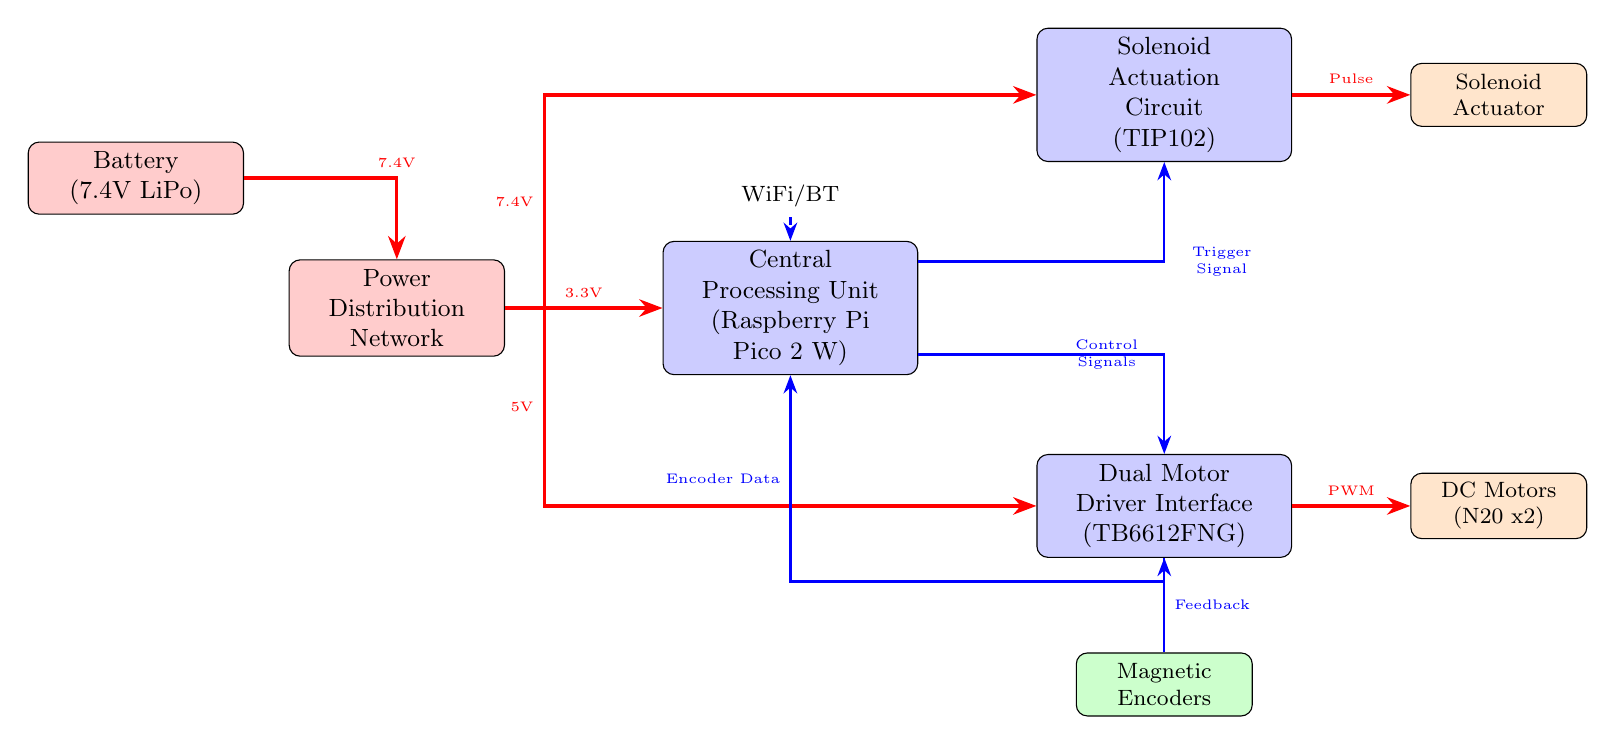
\begin{tikzpicture}[node distance=1.5cm and 2cm,
        block/.style={rectangle, draw, fill=blue!20, text width=3cm, text centered, rounded corners, minimum height=1cm, font=\small},
        power/.style={rectangle, draw, fill=red!20, text width=2.5cm, text centered, rounded corners, minimum height=0.8cm, font=\small},
        sensor/.style={rectangle, draw, fill=green!20, text width=2cm, text centered, rounded corners, minimum height=0.8cm, font=\footnotesize},
        actuator/.style={rectangle, draw, fill=orange!20, text width=2cm, text centered, rounded corners, minimum height=0.8cm, font=\footnotesize},
        arrow/.style={-Stealth, thick},
        powerline/.style={-Stealth, very thick, red},
        dataline/.style={-Stealth, thick, blue}]

    % Power subsystem
    \node[power] (battery) {Battery\\(7.4V LiPo)};
    \node[power, below right=0.8cm of battery] (regulator) {Power\\Distribution\\Network};

    % Central processing
    \node[block, right=of regulator] (mcu) {Central\\Processing Unit\\(Raspberry Pi\\Pico 2 W)};

    % Motor driver
    \node[block, below right=1cm and 1.5cm of mcu] (motordriver) {Dual Motor\\Driver Interface\\(TB6612FNG)};

    % Solenoid driver
    \node[block, above right=1cm and 1.5cm of mcu] (solenoid) {Solenoid\\Actuation\\Circuit\\(TIP102)};

    % Actuators
    \node[actuator, right=1.5cm of motordriver] (motors) {DC Motors\\(N20 x2)};
    \node[actuator, right=1.5cm of solenoid] (sol) {Solenoid\\Actuator};

    % Sensors
    \node[sensor, below=1.2cm of motordriver] (encoders) {Magnetic\\Encoders};

    % Power connections
    \draw[powerline] (battery) -| (regulator) node[midway, above, font=\tiny] {7.4V};
    \draw[powerline] (regulator) -- (mcu) node[midway, above, font=\tiny] {3.3V};
    \draw[powerline] (regulator.east) -- ++(0.5,0) |- (motordriver.west) node[near start, left, font=\tiny] {5V};
    \draw[powerline] (regulator.east) -- ++(0.5,0) |- (solenoid.west) node[near start, left, font=\tiny] {7.4V};
    \draw[powerline] (motordriver) -- (motors) node[midway, above, font=\tiny] {PWM};
    \draw[powerline] (solenoid) -- (sol) node[midway, above, font=\tiny] {Pulse};

    % Data connections
    \draw[dataline] (mcu.340) -| (motordriver) node[midway, left, font=\tiny, text width=1.2cm, align=center] {Control\\Signals};
    \draw[dataline] (mcu.20) -| (solenoid) node[midway, right, font=\tiny, text width=1.2cm, align=center] {Trigger\\Signal};
    \draw[dataline] (encoders) -- (motordriver) node[midway, right, font=\tiny] {Feedback};
    \draw[dataline] (motordriver.south) -- ++(0,-0.3) -| (mcu.south) node[near end, left, font=\tiny] {Encoder Data};

    % WiFi indication
    \node[above=0.3cm of mcu, font=\footnotesize] (wifi) {WiFi/BT};
    \draw[dataline, dashed] (wifi) -- (mcu);

\end{tikzpicture}
\end{document}
